\chapter{Thiết kế}

\section{Mô hình thiết kế}
    Với mục tiêu đề tài giúp các quadcopter bay được ổn định đồng thời vẫn giữ được trạng thái bầy đàn nhóm đề xuất ra mô hình bay như sau:
    \begin{itemize}
    	\item Mô hình sẽ có ít nhất hai chiếc quadcopter có thể hoạt động độc lập ổn định. Như vậy cần có các cảm biến cần thiết để triển khai phương pháp điều khiển PID cho quadcopter. Ngoài ra còn cần mạch thu phát sóng Wifi và một vi xử lý phụ nhằm xử lý dữ liệu bay.
    	\item Trạm điêu khiển mặt đất chạy phần mềm để thiết lập thông số các quadcopter đồng thời hiển thị dữ liệu và điều khiển các quadcopter bay theo các chế độ mong muốn.
    	\item Mỗi chiếc quadcopter kết nối với trạm điều khiển đồng thời trao đổi dữ liệu cảm biến qua lại với nhau nhằm tính toán để giữ đội hình bầy đàn.
    \end{itemize}
    
    \begin{figure}[h!]
    	\begin{center}
    		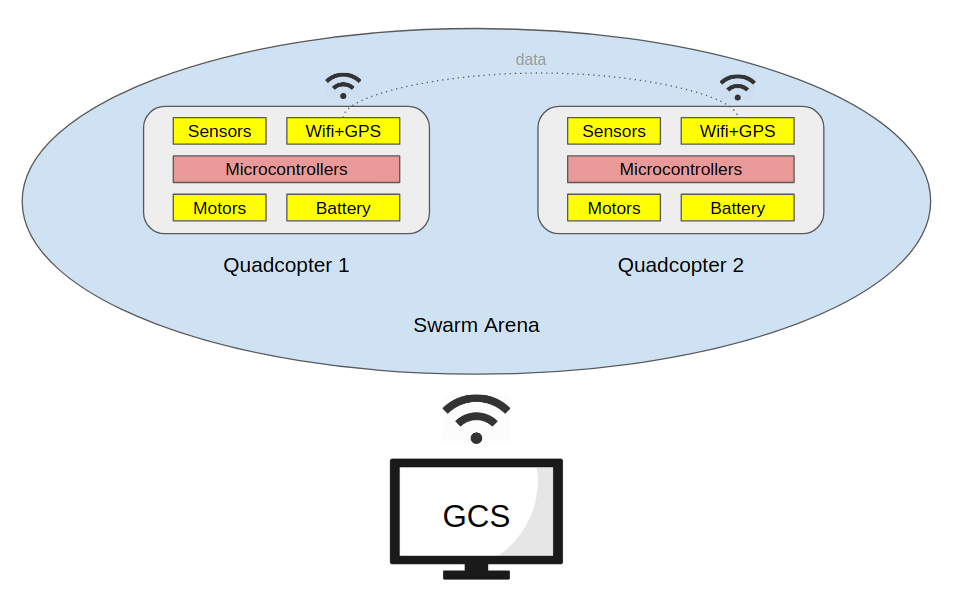
\includegraphics[scale=0.45]{images/design_model.png}
    		\caption{Mô hình thiết kế}
    	\end{center}
    \end{figure}
    
\section{Phần cứng} 
    \subsection{IMU - Đơn vị đo lường quán tính}
    Đơn vị đo lường quán tính là một thiết bị điện tử đo lường lực, tỷ lệ góc và đôi khi là từ trường bao quanh vật thể được dùng. IMU sử dụng kết hợp gia tốc kế, con quay hồi chuyển và từ kế. Nó là một thiết bị không thể thiếu cho các mô hình trên không bao gồm các thiết bị bay không người lái đặc biệt là quadcopter.\\
    Một bộ IMU khác biệt so với dùng các cảm biến riêng lẻ ở chỗ nó bao gồm những tập lệnh được thiết kế cho các phép tính toán ba chiều, tính toán hướng và góc. Mục đích chính là giảm tải thời gian và công suất xử lý cho bộ xử lý trung tâm. Kết quả trả về của nó có thể là giá trị analog hoặc digital đã tính toán tùy chỉnh.
    
    \begin{figure}[h!]
    	\begin{center}
    		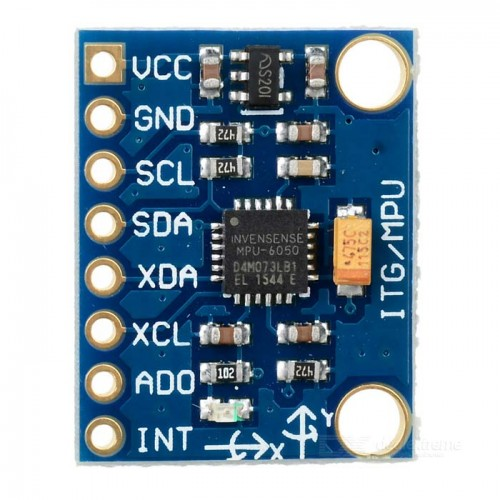
\includegraphics[scale=0.25]{images/mpu6050.jpg}
    		\caption{IMU MPU6050}
    	\end{center}
    \end{figure}
    
    \subsection{MCU - Vi điều khiển}
    Vi điều khiển luôn là bộ não trung tâm của bất kì thiết bị yêu cầu tính toán điện tử nào. Mục đích của vi điều khiển nhằm tạo một môi trường giao tiếp giữa các thiết bị ngoại vi, tính toán và đưa ra số liệu phù hợp để điều khiển các bộ phận giúp quadcopter bay được ổn định. Một vi điều khiển nhằm mục đích điều khiển bay cho quadcopter cần có khả năng xử lý năng lượng thấp, tốc độ xử lý nhanh và nhỏ nhẹ. Ngoài ra nếu muốn hỗ trợ tính toán từ các vi điều khiển khác thì vi xử lý cần có thêm nhiều cổng UART. \\
    Một bộ điều khiển bay Flight Controller là một bo mạch được thiết kế nhỏ gọn tích hợp vi điều khiển và các thiết bị ngoại vi cần thiết như IMU, GPS, ESC hay cảm biến khoảng cách và các cổng kết nối I2C, SPI hay UART. Flight Controller được xây dựng nhằm mục đích giúp người dùng dễ dàng tiếp cận với bộ firmware được xây dựng sẵn cho điều khiển bay cơ bản. Ngoài ra Flight Controller còn hỗ trợ tùy chỉnh thêm linh kiện và firmware cho phù hợp với mục đích sử dụng. \\
    Để đảm bảo quadcopter tính toán nhanh để ổn định mô hình bầy đàn, nhóm sử dụng thêm một vi xử lý phụ để xử lý giữ liệu bay cho các quadcopter.
    
    \begin{figure}[h!]
    	\begin{center}
    		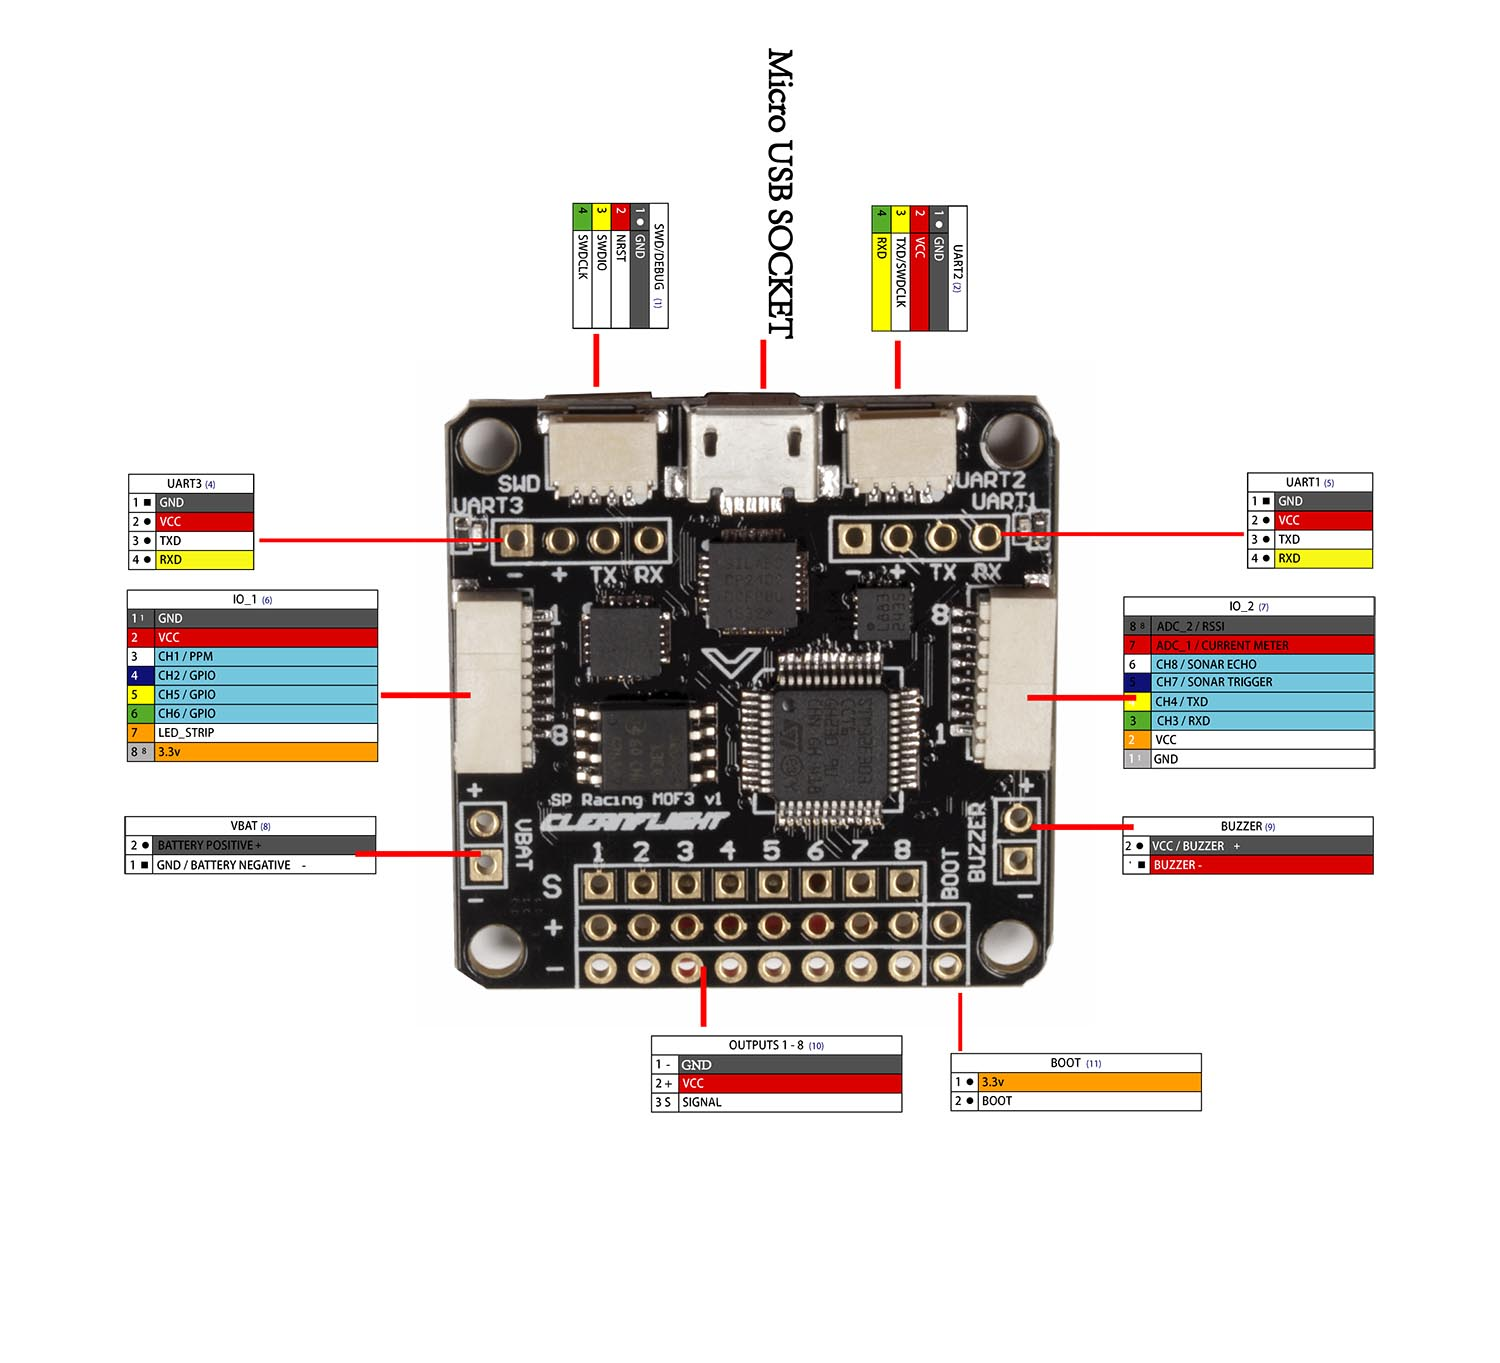
\includegraphics[scale=1.1]{images/sp_racing_f3.jpg}
    		\caption{Flight Controller SP Racing F3 Acro dùng vi xử lý STM32F303}
    	\end{center}
    \end{figure}
    
    \subsection{ESC - Bộ điều tốc}
    Bộ điều tốc ESC (Electronic Speed Control) là một bo mạch dùng nguồn điện ba pha điện áp thấp từ nguồn DC để thay đổi tốc độ động cơ không chổi than (brushless), chiều quay và cũng có thể sử dụng như thắng điện tử cho động cơ. Động cơ không chổi than là động cơ với công suất tiêu thụ cao chuyên dùng cho quadcopter hay những thiết bị cần công suất tiêu thụ cao khác và chạy với thời gian thực. 
    
    \begin{figure}[h!]
    	\begin{center}
    		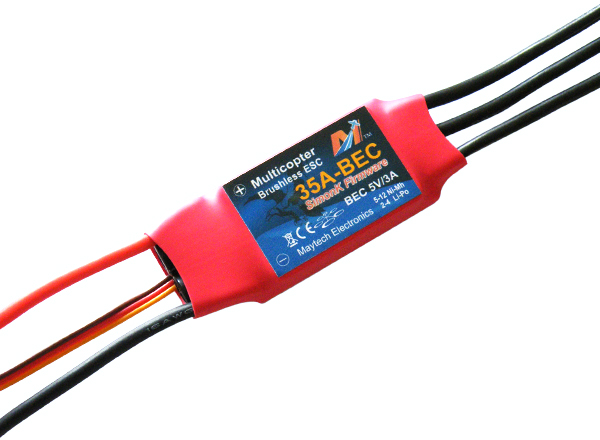
\includegraphics[scale=0.4]{images/esc.jpg}
    		\caption{Multicopter Brushless ESC 35A-BEC 5V/3A}
    	\end{center}
    \end{figure}
    
    \subsection{ESP8266}
    ESP8266 là dòng chip tích hợp Wi-Fi 2.4Ghz và một vi xử lý tốc độ 80MHz với chi phí thấp. ESP8266 vừa dùng để làm module giao tiếp giữa các quadcopter với nhau vừa có thể dùng để giao tiếp với trạm điều khiển mặt đất.

    \begin{figure}[h!]
    	\begin{center}
    		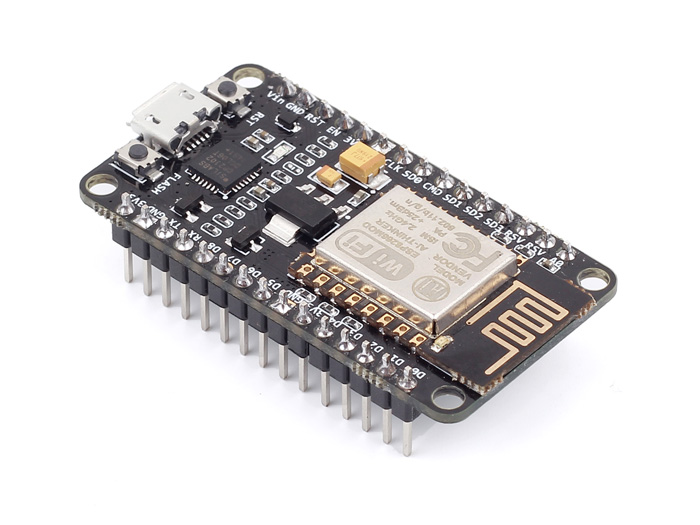
\includegraphics[scale=0.2]{images/esp8266.jpg}
    		\caption{NodeMCU ESP8266 WiFi ESP-12E}
    	\end{center}
    \end{figure}
    
    \subsection{Ultrasonic Sensor - Cảm biến siêu âm}
   Cảm biến sóng siêu âm được sử dụng rất phổ biến để xác định khoảng cách bởi giá thành rất rẻ và độ chính xác cao. Cảm biến siêu âm có thể đo khoảng cách trong khoảng từ 2cm đến 300cm dùng sóng siêu âm.
   Trong mô hình quadcopter, cảm biến siêu âm được xếp đều xung quanh quadcopter để giữ khoảng cách với vật cản và các quadcopter khác.
   
   \begin{figure}[h!]
    	\begin{center}
    		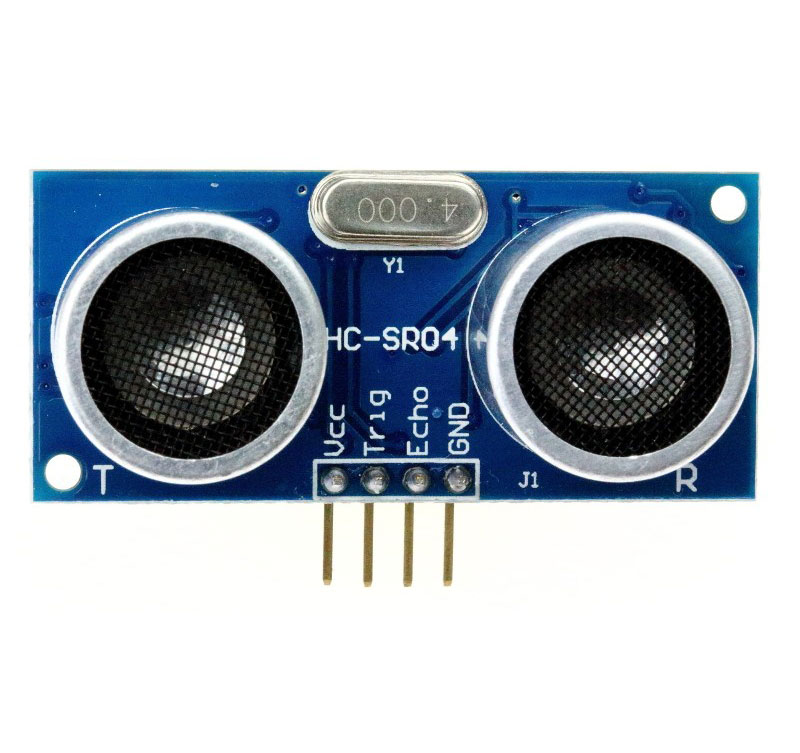
\includegraphics[scale=0.1]{images/ultrasonicsensor.jpg}
    		\caption{Ultrasonic Sensor HC-SR04}
    	\end{center}
    \end{figure}
   
    \section{Chương trình điều khiển và mô phỏng}
            \subsection{ArduCopter}
            ArduCopter là một hệ thống tự lái nâng cao mã nguồn mở cho các thiết bị bay dùng một hay nhiều rotor. Nó cung cấp nhiều chế độ bay từ thủ công cho đến bay hoàn toàn tự động.\\
            ArduCopter là một nhánh của chương trình rộng hơn ArduPilot cung cấp cho nhiều loại phương tiện bay trên không. Nó hoạt động liền mạch với chương trình điều khiển từ mặt đất được dùng để cài đặt phương tiện, hiển thị dữ liệu thời gian thực từ chuyến bay và lên kế hoạch bay cho phương tiện. Hệ sinh thái ArduPilot còn đem đến nhiều tính năng khác như mô phỏng bay, các công cụ phân tích nhật ký hành trình và các API nâng cao cho việc điều khiển phương tiện.\\
            Mục tiêu của nhóm là phát triển thêm chế độ bay theo bầy đàn dựa trên mã nguồn của ArduCopter và tiến xa hơn là chương trình điều khiển từ mặt đất với giao diện người dùng dễ sử dụng.
    
    \begin{figure}[h!]
    	\begin{center}
    		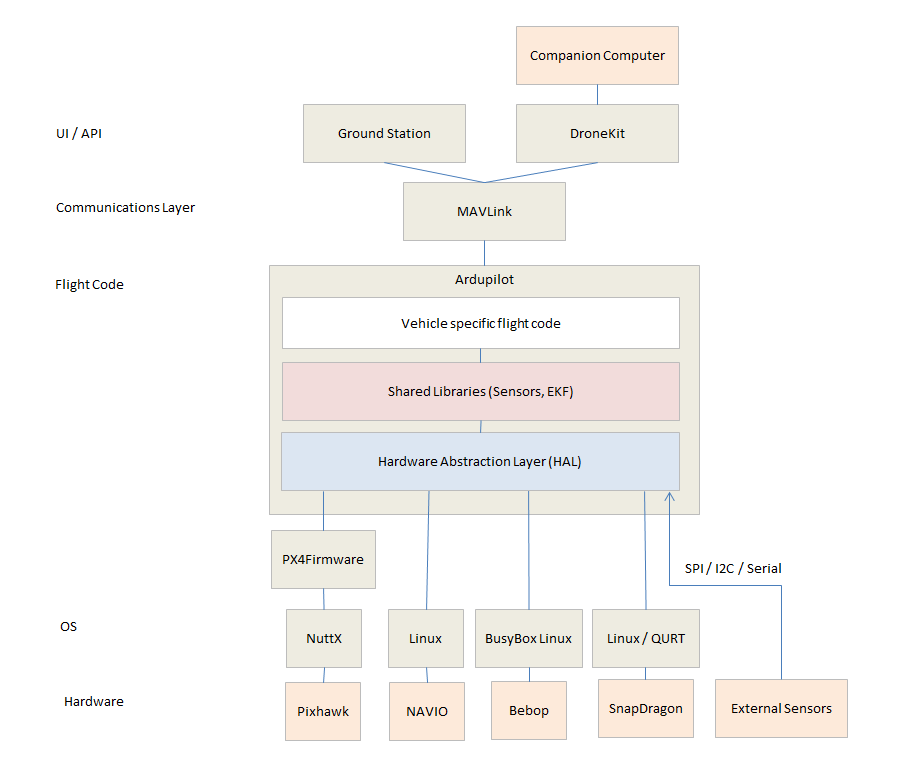
\includegraphics[scale=0.5]{images/ArduPilot_HighLevelArchecture.png}
    		\caption{Kiến trúc của Ardupilot}
    	\end{center}
    \end{figure}

			Cấu trúc cơ bản của ArduPilot gồm 5 phần chính:
			\begin{itemize}
    	\item Mã lập trình phương tiện (Vehicle code)
    	\item Các thư viện được chia sẻ (Shared libraries)
    	\item Lớp trừu tượng phần cứng (Hardware abstraction layer)
    	\item Các công cụ (Tool directories)
    	\item Các mã lập trình hỗ trợ ngoài (External support code: MAVLink, DroneKit)
    		\end{itemize}
    		
    		Như vậy nhóm sẽ tập trung vào phần lập trình quadcopter là mã nguồn ArduCopter. Cụ thể là viết phần chế độ bay theo bầy đàn ở lớp \textit{Mode} và file mã nguồn chế độ bay là \textit{Mode.cpp}.
    		
    \begin{figure}[h!]
    	\begin{center}
    		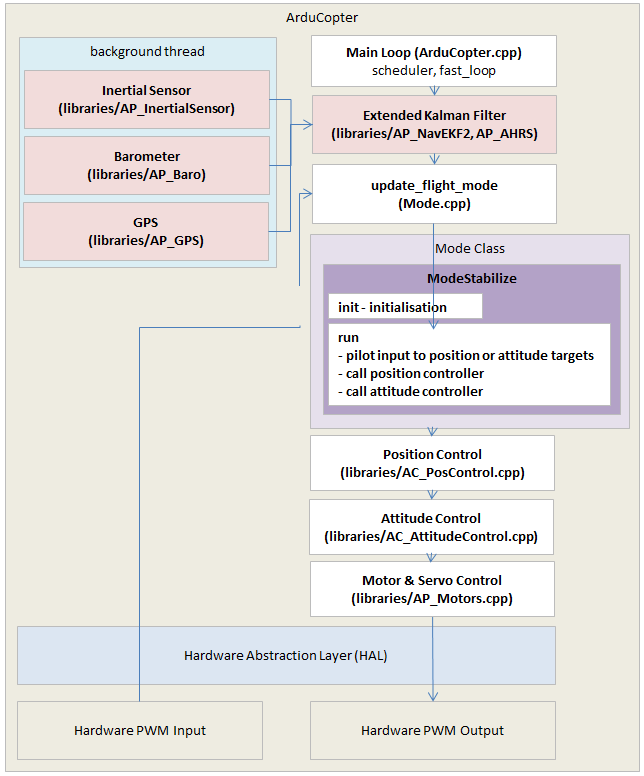
\includegraphics[scale=0.6]{images/copter-architecture.png}
    		\caption{Kiến trúc mã nguồn ArduCopter}
    	\end{center}
    \end{figure}
    
    \subsection{SITL Simulator}
    		Ardupilot cung cấp công cụ mô phỏng bay SITL (Software in the loop) cho phép mô phỏng bất kì phương tiện nào mà không cần đến phần cứng. Nó là một bản build từ mã nguồn Ardupilot chính nhưng cung cấp các thông tin phần cứng ảo. Lợi ích lớn nhất của SITL là cho phép sử dụng toàn bộ các công cụ phát triển bằng ngôn ngữ C++ trên máy tính như các trình gỡ rối, công cụ phân tích dữ liệu hay mô phỏng không gian ba chiều giúp khả năng phát triển và kiểm thử tính năng mới trên ArduPilot trở nên đơn giản hơn. 
    		
    \begin{figure}[h!]
    	\begin{center}
    		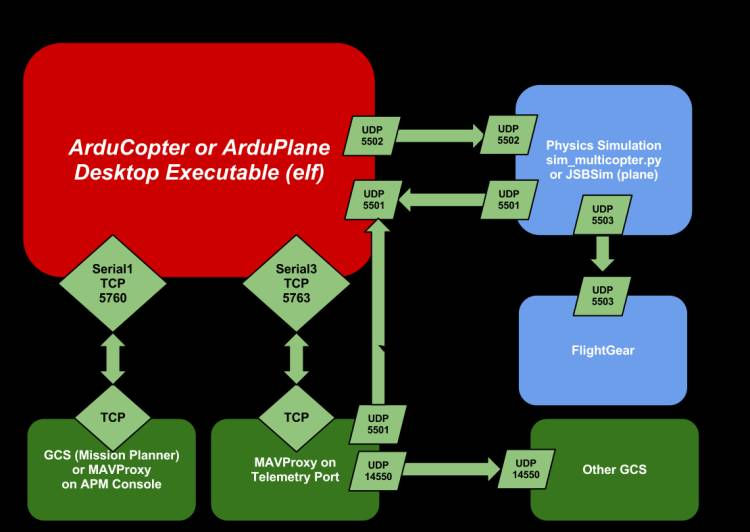
\includegraphics[scale=0.35]{images/ArdupilotSoftwareintheLoopSITL.jpg}
    		\caption{Kiến trúc phần mềm mô phỏng SITL}
    	\end{center}
    \end{figure}
    
    \begin{figure}[h!]
    	\begin{center}
    		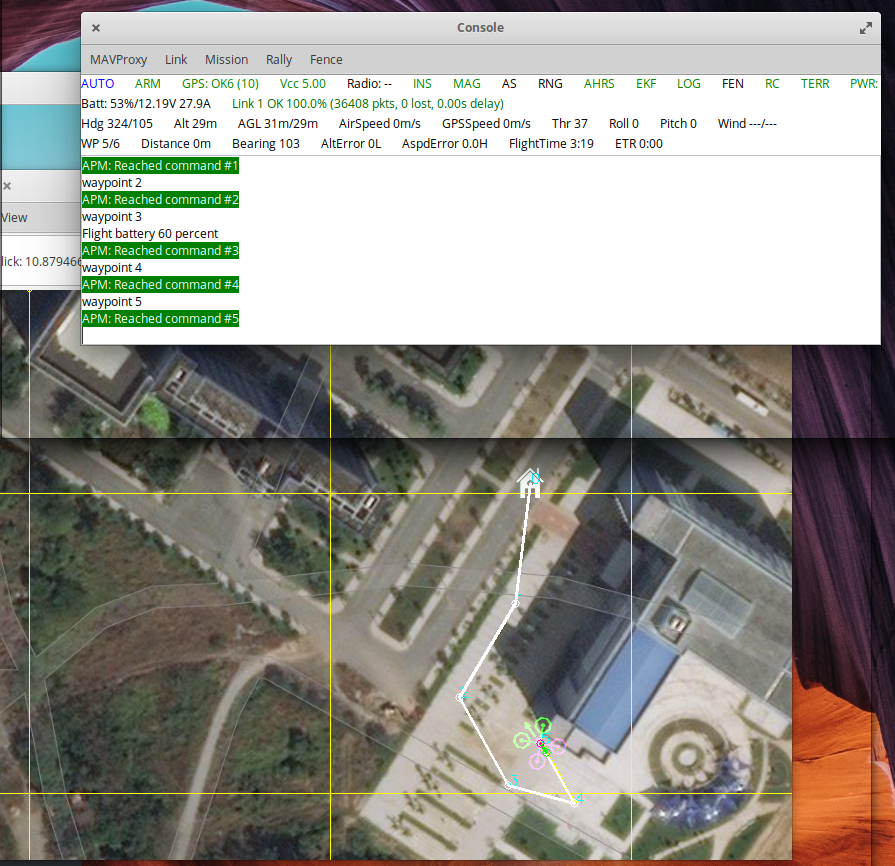
\includegraphics[scale=0.45]{images/simulating.png}
    		\caption{Mô phỏng một quadcopter bay theo quỹ đạo ở BKU cơ sở 2}
    	\end{center}
    \end{figure}